\columnbreak
\part{Data Interpolation in 1D}
\setcounter{section}{0}

%Goal
\textbf{Goal:} Given data points $(t_i, y_i)$ and a finite-dimensional vector-space of functions $V$, reconstruct $f\in V$ such that $\forall i \quad f(t_i)=y_i$. \\

\Def[Interpol. as linear mapping] \\
For data points $(t_i, y_i) \quad i=0,\dots,n$
and $V$ spanned by basis functions $b_0,\dots b_m$ we have
$$
\mathbf{A} \mathbf{c}:=\left[\begin{array}{ccc}
b_{0}\left(t_{0}\right) & \ldots & b_{m}\left(t_{0}\right) \\
\vdots & & \vdots \\
b_{0}\left(t_{n}\right) & \ldots & b_{m}\left(t_{n}\right)
\end{array}\right]\left[\begin{array}{c}
c_{0} \\
\vdots \\
c_{m}
\end{array}\right]=\vy
$$
$\rightarrow$ The interpolant is uniquely solv. iff $m=n$\\
$\rightarrow$ The basis is \textbf{cardinal} if $b_{j}\left(t_{i}\right)=\delta_{i j}$

\section{Global Polynomial Interpol.}

\Def[Monomial Basis]\\
$\rightarrow$ Evaluation in $\BigO(n)$ by exploiting associativity.

\Def[Lagrange Basis]\\
$$L_{i}(t):=\prod_{j=0 \atop j \neq i}^{n} \frac{t-t_{j}}{t_{i}-t_{j}} = I_\mathcal{T}(\ve_{i+1})$$
$\rightarrow$ Cardinal Basis.
\sep

\section{Shape-Preserving Interpol.}

\Method[Piecewise linear Interpol.] \\
$\rightarrow$ locally shape preserving \\
Tent functions make a cardinal basis:
\begin{center}
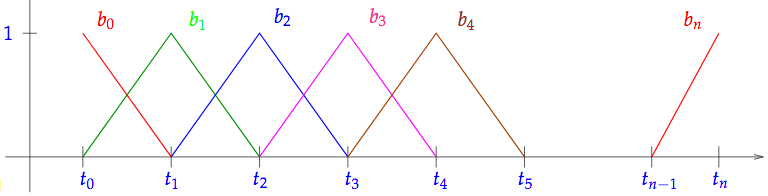
\includegraphics[height=25px, width=\columnwidth,]{5_tent.png}
\end{center}

\section{Splines}
\section{Trigonometric Interpol.}
\section{Least Squares Fitting}


-> efficient interpolation at many points O(n^2 + N * n)

-> Aitken-Neville for single point evaluation in O(n^2), 
	useful for simoultatneous updates, update in O(k), eval in O(1).
	
- Extrapolation 
-> Algorithm to extrapolate to zero

Barycentric Algorithm:
- Precomputation: O(n^2)
- eval at single spot in O(n)

Aitken-Neville (SINGLE POINT EVALUATION:
- update in in O(k).

Newton Basis: 
- Precomputation: add node in O(n)
- eval at a single spot in O(n)

-> Divided Differences algorithm for newton basis (computes in situ, hence better than forward substitution)

 sensitivity vs stability
 -> lebesque?
 
 ## Shape-preserving Interpolation -> Cubic Hermite Interpolation:
 -> Interpolate as piecewise polynomial, where ends mach (derivative)
 Different methods to determine properties of piecewise borders:
 	- Linear (Derivative is weighted mean of adjacent derivatives) -> No Preservation of monotonicity
 	- Limited Slopes (Pchip): Since slope must be zero at boundary in some cases -> Not linear
 	
 ## Splines (see wooden splines!)
 -> Instead of fixing the boundary slopes, we add additional continuity conditions. We need to add exactly n+1 conditions.
 #### Cubic Splines
 -> n-1 conditions given by saying SECOND derivate must be the same.
 The remaining two conditions can be:
	natural -> leftmost and righmost zero
	periodic -> leftmost and righmost must match
	full -> we dictate conditions on lefmost and rightmost border
	
Note that:
	- cubic splines are not shape preserving
	- cubic splines are weakly local
	
	
See 5.4.2.1 for a comparison of methods.

